% Chapte 8 
\chapter{Interactive and non Interactive on site study} % Main chapter title

\label{Chapter8} % For referencing the chapter elsewhere, use \ref{Chapter1} 

\section{Introduction}

The On-sight study is going to be executed in Weimar tourist Information Center at (Weimar Markt 10) which is one of important location for many tourists who visit Weimar. This location was chosen by Bauhaus-Spaziergang program that are providing tours for new visitors in Weimar. Bauhaus-Spaziergang does advertisement as brochure at this location. The location is reserved for our new interactive advertisement starting from 1st February for three coming weeks. 

Two different Interactions and one non-Interactive Advertisement are made. The first one is body interaction where passers-by can interact using their body movement in the physical space and influence advertisement element in the screen. The second is mobile interaction where users by opening the advertisement web application in their smartphone, can interact with advertisement and the third is a non-interactive advertisement where the interface and elements are completely similar but are not influence by people around, they change based on time-based random sequence. 

\section{Interactive Advertisement}

\subsection{Body Interactive}

\subsection{Mobile Interactive}

\section{Auto Interactive Advertisement}


\section{Problem Statement}



\section{Problem Statement}
\begin{enumerate}

\item	For which of the three conditions (body, mobile and non-interactive advertisements) passers-by 

\begin{enumerate}
\item	Are more attracted toward.
\item	Perform Honeypot and Landing effects.
\item	Are engaged with the screen.
\item	Spend extra time for watching the remaining advertisement video after interaction.
\end{enumerate}

\item   Find out potential conversion rate toward the Bauhaus-Walk program.
\item	How many people understand advertisement?
\item	Get general opinion about the advertisement techniques.
\item	Comparison of Mobile and body interaction techniques.

\end{enumerate}







\section{Design study}


\subsection{Duration}
Each type of advertisement were installed for one five days 


\subsection{Location}
The screen was installed in Weimar Tourist Information center. This center is one of the famouse tourist information in Weimar where alot of tourists visit. Most importantly this location was chosen because our target audience (tourists) mainly elders visit.


\subsection{Participants}
The participants were the ones who passby the screen, non of the participants were informed about this study nor any notes were put at the entrance. Roughly \%60 of the participants were elder aged between 30-60, \%25 were young and the rest \%15 were children.


\subsection{Advertisement week sequence}

\begin{table}[H]
\caption{Week sequence}
\label{tab:advertisementWeeks}
\centering
\begin{tabular}{l l l l }
\toprule
\tabhead{Advertisement} & \tabhead{1st Week} & \tabhead{2nd Week} & \tabhead{ 3rd Week} \\
\midrule
\textbf{Auto Interactive}     &   X    &         &     \\
\textbf{Body Interactive}     &        &    X    &    \\
\textbf{Mobile Interactive }  &        &         &   X   \\
\bottomrule\\
\end{tabular}
\end{table}



\section{Data gathering}
Several types of data from different aspects were gathered for each individual week to be able for analyzing and also be able to answer new arising questions after the onsite evaluation, the bellow types of data were gathered.


\begin{enumerate}
\item \textbf{On-Site Observation} \\
Observation periods were arranged in two different time slots per day, the first time slot was from 10:00 – 12:00 and the second was from 14:00 – 16:00, except for Saturday and Sunday where the tourist information center was open only until 14:00, then the observation period was from 10:00-12:00 and 13:00-14:00. During these two time slots the bellow observations were made and to remove the effects of specific time order,the orders were counterbalanced.

\begin{enumerate}
\item \textbf{Attention Level measurement} \\
Attention level is how much a person gives attention to the display, which consist of number of glances and number of ignores and how much long a person is standing infront of the display.At the beginning gaze-tracking method was considered for accurate measurement of attention level, a very impressive work have been done from Intraface \cite{Intraface} that can not only detect glances but also human emotions at the time, but because of high flow rate that method was not used and instead the glance counting which was proposed by \cite{glancingcount} that has formalized a ranking system from which  glance is considered if a person reacts to the display by turning his/her head toward it that last less than 3 seconds.

One hour attention level counting for each time slot was conducted, in which the observer was writing the number of people passing by and how many of them glanced and ignored the screen.see the glance counting sheet in Appendix: \ref{AppendixA}.1

\item \textbf{Passerby behavior and Interviews} \\
During one hour per time slot per day the passerby behavior were observed like how they approach to the screen, how do they react, what path the passerby take and what are they looking for and even how they ignore the display and after they are done with the screen engagement a very short interview was taken from them. 

\end{enumerate}


\item \textbf{System Logs} \\
The Advertisement application can generate the bellow logs.
\begin{enumerate}

\item	\textbf{Non-Interaction application} \\
Only duration(seconds) spent in front of the display is logged for each individual person.

\item	\textbf{Interaction application}\\
For this type the system can detect

\begin{itemize}
\item	Time user joins.
\item	Interaction completion time.
\item	Number of tasks (locations) explored.
\item	Whole duration spent(sec).
\item	If the user has seen advertisement or not.
\end{itemize}

\end{enumerate}

\item \textbf{Interviews} \\
Interviews were taken from the passerby that had some sort of engagement with the display like for non-interactive advertisement the people were interviewed that they stood for a while and saw the advertisement and for the interactive advertisement the people were interviewed that interacted or tried to interact with the system.
A leaflet, that describes the thesis goal and interview consent form was handed to the participants and after signature the interview was conducted. All the interviews were audio recorded and later transcribed for analysis, all interviews took in average 4 minutes, the reason we took short interviews was that most of the people were tourists and had little time to stay and even some of them rejected interview because of shortage of time.
Each week there were some variation in the questions dependent to the type of advertisement.  See appendix \ref{AppendixD}.1


\item \textbf{Depth recordings} \\
Depth recording from Kinect camera was done during entire three weeks for non-interactive and interactive advertisement for many reasons.

\begin{itemize}
\item Match the log data with the video data for accuracy.
\item Measure the number of Honeypot effects and landing effects.
\item Observe passerby behavior in detail.
\end{itemize}

Because of limited space and processing power, the actual depth information (x,y,z) for individual points was not stored but a 2D colored image was taken per second and after the image recording was done, in lab another post processing script was applied to integrate a static background using Adobe Photoshop application. To match the data logs and the image frames each image name consisted the date and time as (10.12.43.21.png).

\begin{figure}[!htb]
    \centering
    \subfloat[]{{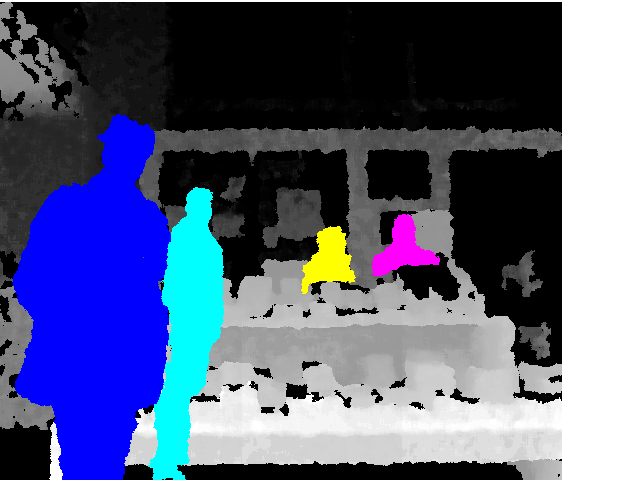
\includegraphics[width=50mm,height=40mm]{Figures/8/d1} }}%
    \subfloat[]{{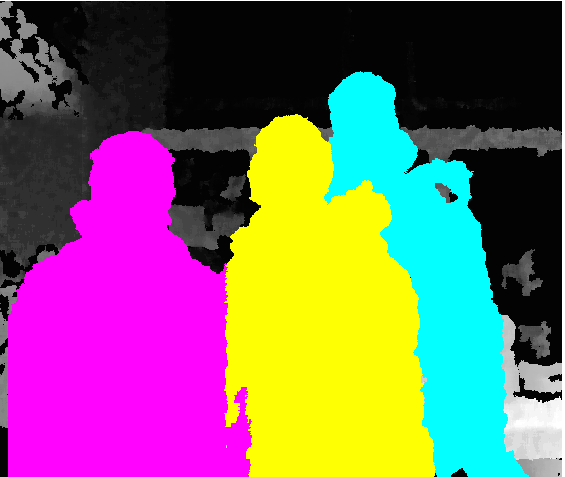
\includegraphics[width=50mm,height=40mm]{Figures/8/d2} }}%
    \caption{Depth recording examples}%
    \label{fig:DepthRecordedImages}%
\end{figure}

\end{enumerate}

Other pictures were also taken using mobile phone from the scene, verbal permission were taken before the photographing them.



\section{Data Analysing}


\subsection{Individual week analysing}


\begin{enumerate}

\item Glance counts \\
The glance counts were transformed from paper to spreadsheet in which number of glances and ignores were recorded individually and then combined from which mean value and percentages are extracted. see Appendix \ref{AppendixD}.2, \ref{AppendixD}.3 and \ref{AppendixD}.4 for each week.

\item Interviews \\
All the interviews were transcribed and color coded from which interesting categories had emerged, each code is separately discussed in the finding section, To see color coded diagram see Appendix \ref{AppendixD}.5, \ref{AppendixD}.6 and \ref{AppendixD}.7 for each week


\item Display Engagement phases and time \\
Log files along depth images were seen and compared to have accurate values for each engagement phases and the whole interaction phases. depth frames were manually frame-by-frame analysed and the logs were cleared from any possible mistakes.

\item Honeypot and landing effects \\
These two effects were observed mainly from the depth frames and also partially from onsite observation.


\end{enumerate}


\subsection{Comparison of different advertisement}



\section{Findings}



\subsection{Individual advertisement}


\subsubsection{Non-Interactive findings}

\begin{enumerate}
\item Attention Level measurements


\begin{figure}[H]
    \centering
    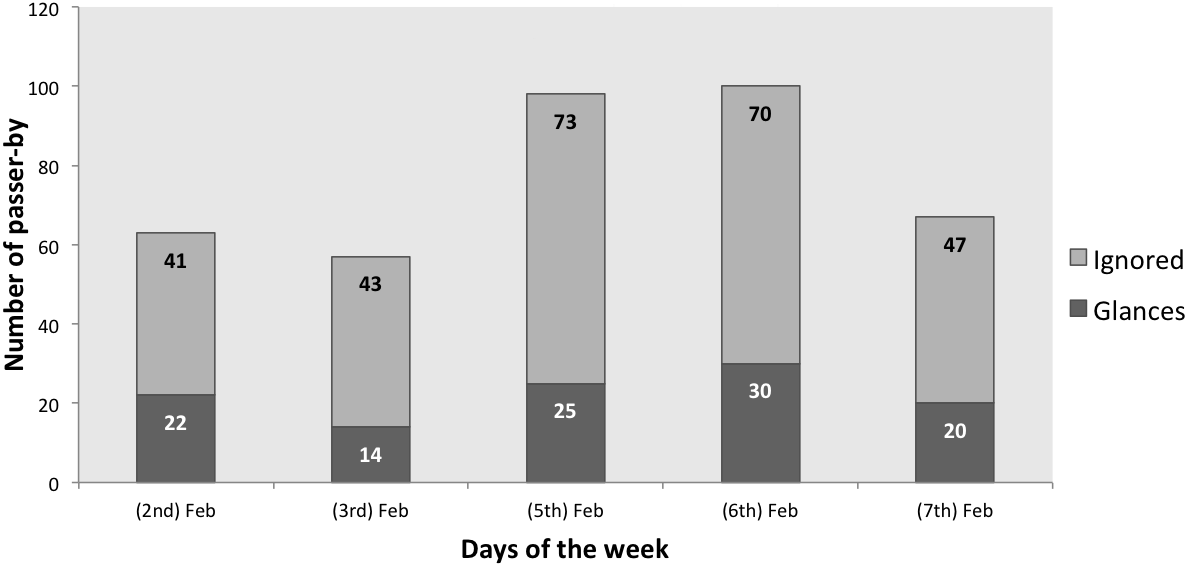
\includegraphics[width=110mm,height=55mm]{Figures/8/non_inter_findings/Non_Inter_chart}%
    \caption{Non-interactive attention level chart}%
    \label{fig:Nonattentionlevelchart}%
\end{figure}



\begin{figure}[H]
    \centering
    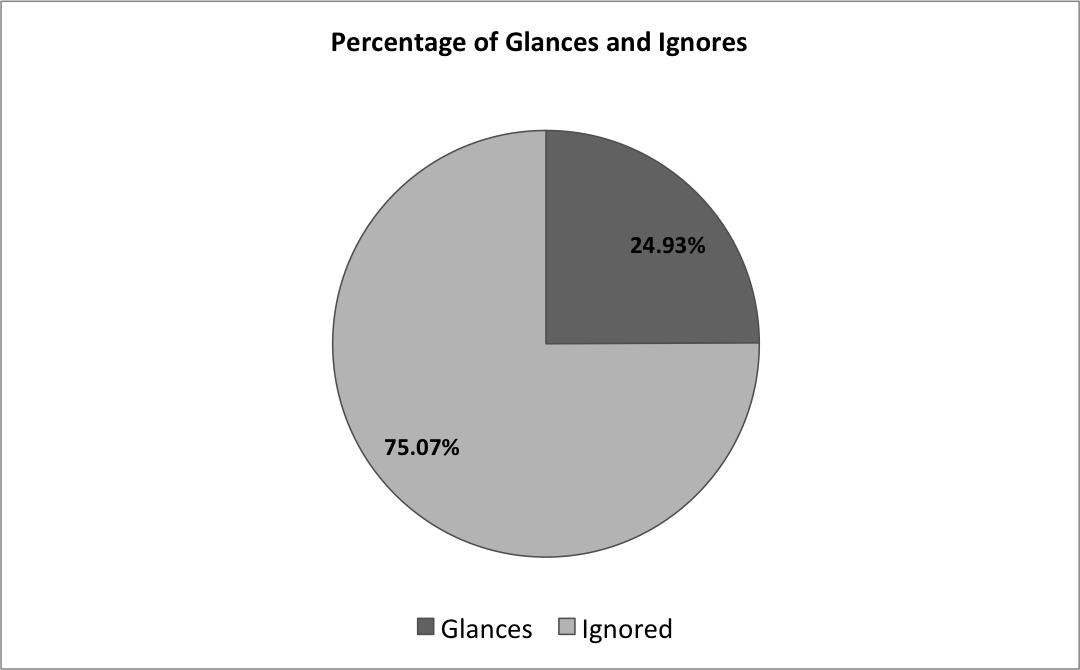
\includegraphics[width=110mm,height=55mm]{Figures/8/non_inter_findings/non_inter_percentage}
    \caption{Non-interactive Attention level percentage}%
    \label{fig:Nonattentionlevelpercentage}%
\end{figure}



\item Engagement time
The average engagement time was about 34.02 seconds.

\item Passerby and engagement


\begin{figure}[H]
    \centering
    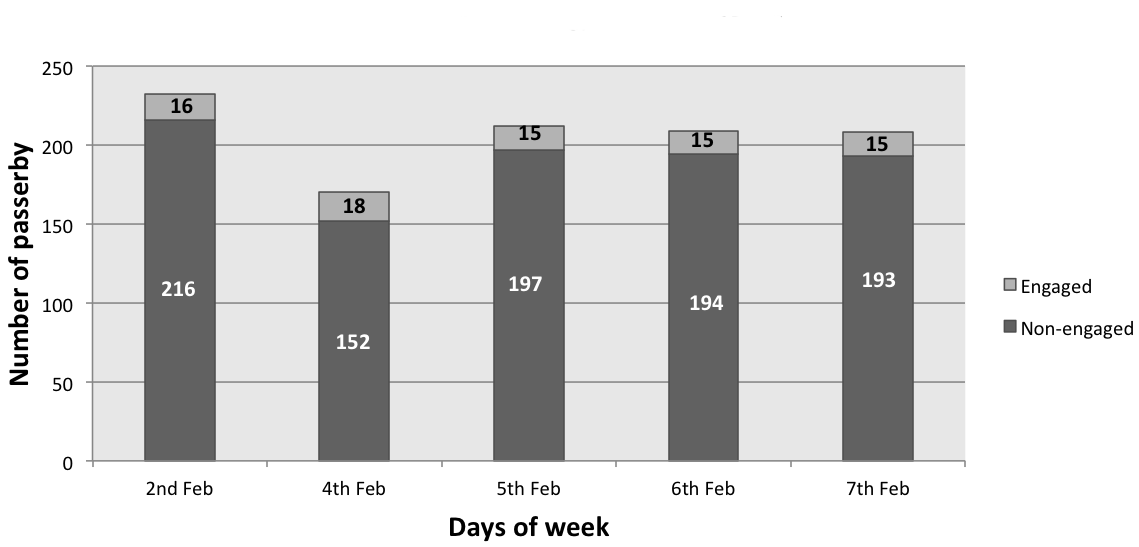
\includegraphics[width=110mm,height=60mm]{Figures/8/non_inter_findings/non_inter_engage_day}
    \caption{Non-interaction Number of engaged passerby}%
    \label{fig:Nonengagedandengagedby}%
\end{figure}

\begin{figure}[H]
    \centering
    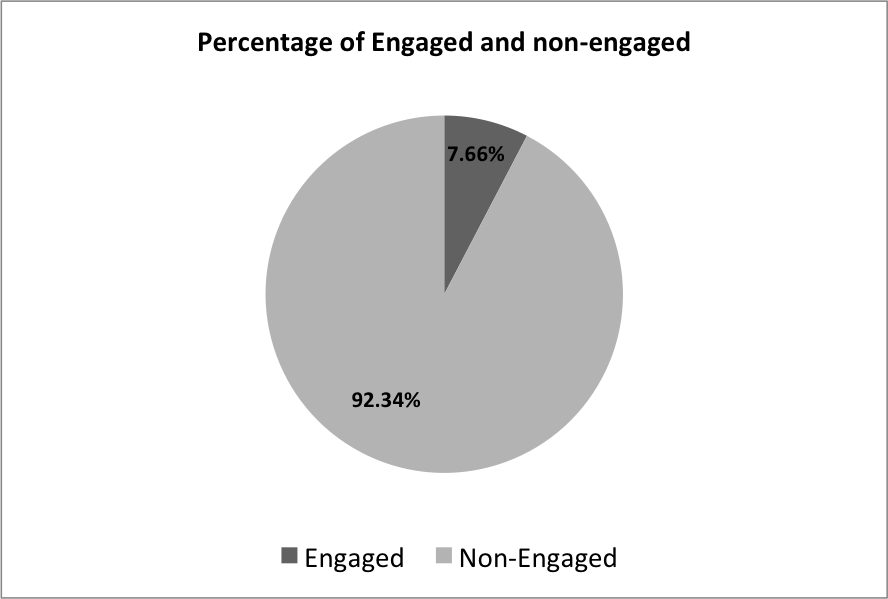
\includegraphics[width=110mm,height=60mm]{Figures/8/non_inter_findings/non_eng_percentage}
    \caption{Percentage of engaged and passerby}%
    \label{fig:Nonengagedpasserbypercentage}%
\end{figure}


\item Landing and Honeypot effects

\begin{table}[H]
\caption{Landing and honeypot effects}
\label{tab:landingandhonypot}
\centering
\begin{tabular}{| l | c | c |}
\toprule
\tabhead{Days} & \tabhead{Landing effect} & \tabhead{Honeypot effect} \\
\midrule
\textbf{2nd Feb}  & 1 &  1 \\
\textbf{4th Feb}  & 0 &  1 \\
\textbf{5th Feb}  & 2 &  3 \\
\textbf{6th Feb}  & 0 &  3 \\
\textbf{7th Feb}  & 1 &  1 \\
\bottomrule
\end{tabular}
\end{table}

\item Interview

\begin{enumerate}

\item Likes \\
Many things from the advertisement were interesting, like the concept of map and the design. As one stated that, ``\emph{I find the idea good, it is nice to see the pictures of the places on the map}'', ``\emph{it is very nice idea because it will be remembered and when I go to the city I will remember}''

\item Dislikes \\
Most of the respondents complained on the speed of the advertisement that how fast the image changes as one said ``\emph{But the pictures were changing very fast}'' other said, ``\emph{advertisement is a little fast}'' They mentioned that why speed is an issue as stating, ``\emph{we wanted to see the map}'', ``\emph{ Could not read the text}''. Many things were disliked by some of the respondents like the advertisement theme, one said, ``\emph{It did not have Bauhaus Theme, the color and that design}'' One respondent also disliked the blinking points.

\item  Participation \\
Respondents mentioned the same excuses that were given at body interactive advertisement, one said, ``\emph{I will join if I am free}'', other said, ``\emph{I have no time}'', or ``\emph{if the weather is good}''. 

\item  Advertisement recall
People could recall the ad, as one mentioned, ``\emph{It is for a tour of Bauhaus in Weimar}'' other said, ``\emph{People can visit the city}'' and some mentioned directly the name of the program ``\emph{Bauhaus-Spaziergang}''.

\item Recommendations \\
There were many recommendations proposed by the responders, which was on content, speed, design.Content related recommendations was that one said, ``\emph{If the prices are mentioned it would be good so that they can decide if they want to take it or not}'' other said on timing, ``\emph{how long does this tour take so people arrange their}''. Another mentioned on speed like ``\emph{it must be little slow}''.

\end{enumerate}


\item Note taking


See appendix  \ref{AppendixD}.8


\item Other observations

Discuss on bellow things

Approaching to the screen

describe the other pictures you have saved in the folder


\end{enumerate}


\subsubsection{Body Interactive findings}

\begin{enumerate}
\item Attention Level measurements


\begin{figure}[H]
    \centering
    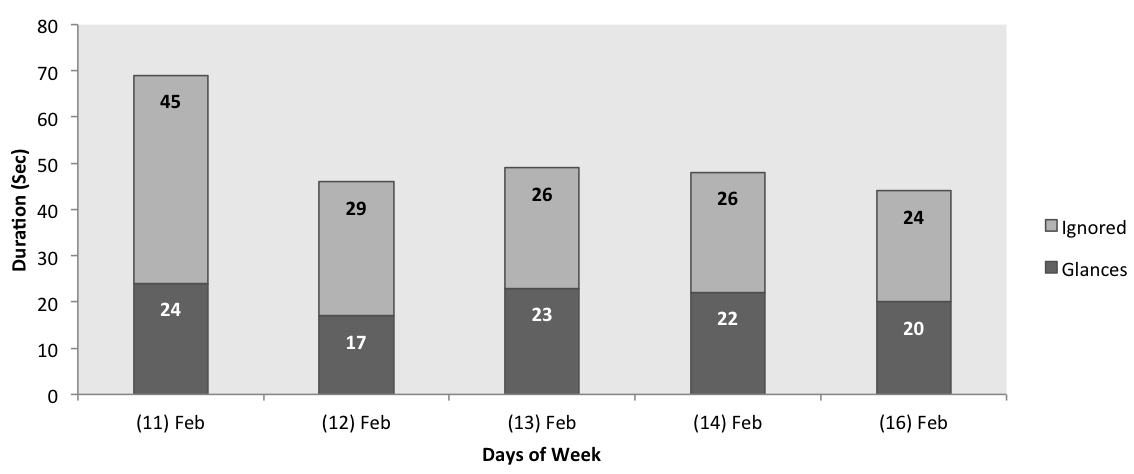
\includegraphics[width=110mm,height=60mm]{Figures/8/body_inter_findings/Body_Inter_chart}%
    \caption{Body interactive attention level chart}%
    \label{fig:bodyattentionlevelchart}%
\end{figure}


\begin{figure}[H]
    \centering
    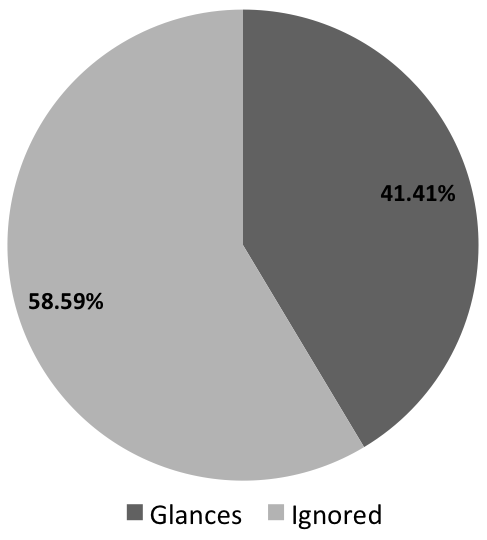
\includegraphics[width=110mm,height=60mm]{Figures/8/body_inter_findings/body_inter_percentage}
    \caption{Body interactive Attention level percentage}%
    \label{fig:bodyattentionlevelpercentage}%
\end{figure}



\item Engagement time

41.84 sec are spent in average



\item Engagement phases

\begin{figure}[H]
    \centering
    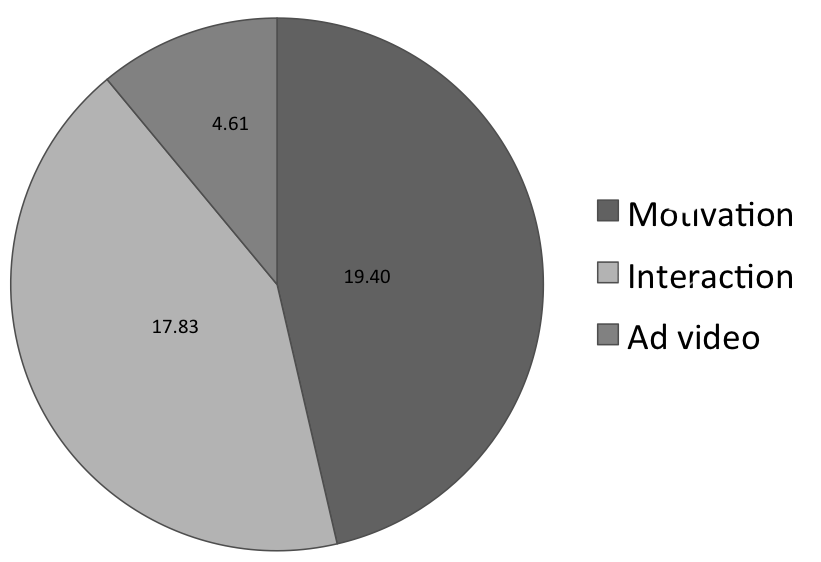
\includegraphics[width=110mm,height=60mm]{Figures/8/body_inter_findings/body_avg_phases}
    \caption{Average time for each phase}%
    \label{fig:bodyaveragephases}%
\end{figure}



\item Passerby and interactions

\begin{figure}[H]
    \centering
    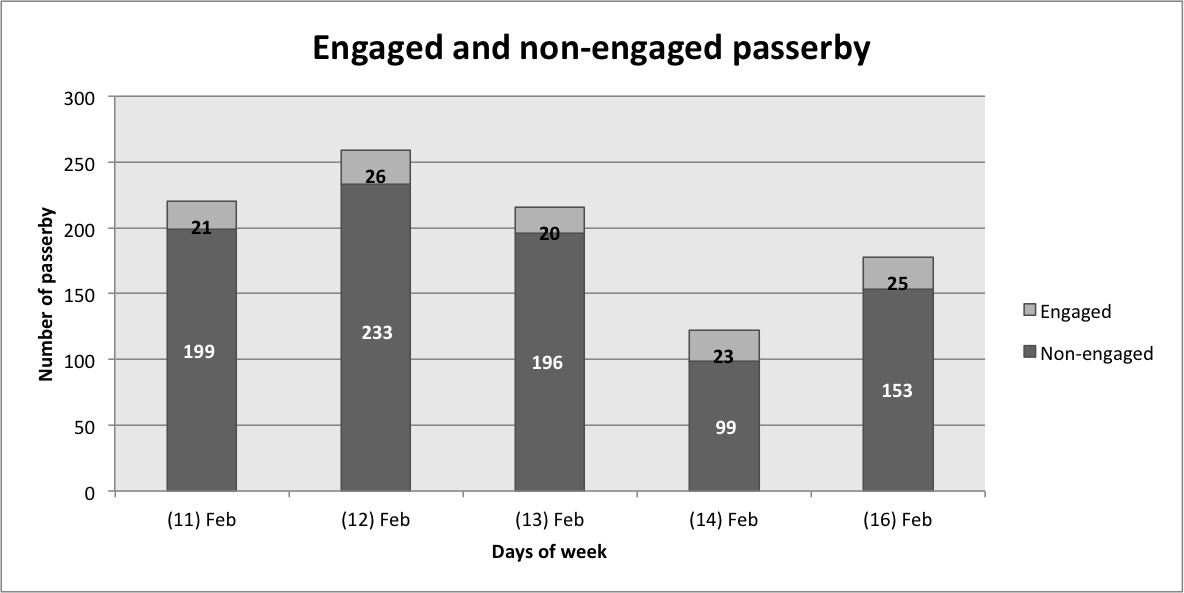
\includegraphics[width=110mm,height=60mm]{Figures/8/body_inter_findings/body_inter_engage_day}
    \caption{Body interactive Number of engaged passerby}%
    \label{fig:bodyengagedandengagedby}%
\end{figure}

\begin{figure}[H]
    \centering
    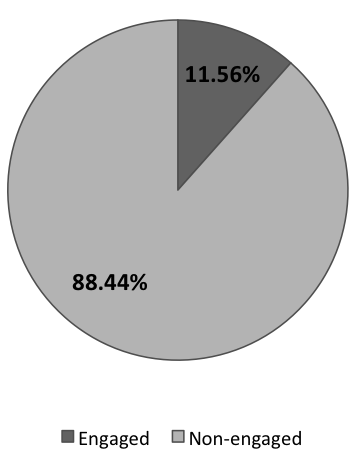
\includegraphics[width=110mm,height=60mm]{Figures/8/body_inter_findings/body_eng_percentage}
    \caption{body interactive percentage of engaged passerby}%
    \label{fig:bodyengagedpasserbypercentage}%
\end{figure}


\item Landing and Honeypot effects

\begin{table}[H]
\caption{Body Interactive Landing and honeypot effect}
\label{tab:landingandhonypot_body}
\centering
\begin{tabular}{| l | c | c |}
\toprule
\tabhead{Days} & \tabhead{Landing effect} & \tabhead{Honeypot effect} \\
\midrule
\textbf{11 Feb}  & 2 &  2 \\
\textbf{12 Feb}  & 3 &  3 \\
\textbf{13 Feb}  & 2 &  2 \\
\textbf{14 Feb}  & 2 &  5 \\
\textbf{16 Feb}  & 3 &  3 \\
\bottomrule
\end{tabular}
\end{table}


\item Interview


The interviews were coded each individually and as a result the bellow categories are extracted, these categories are mainly taken from the questions and others are from the replies of the participants. 

\begin{enumerate}

\item Noticing \\
    Different people had their different experience and reaction when they noticed themselves in the display for the first time. Some of the people were standing and looking some books for long time when they saw themselves and for confirmation they waved toward the screen, as one said ``\emph{Yes at first I thought that it is not me. I waved my hand and came near.}'' Other said, ``\emph{Yes I saw my blue color body}''. Other participants noticed at the time of passing from front of the screen, ``\emph{when I was passing I saw myself in the screen.}'' Other people saw their friend first then noticed themselves like one said, ``\emph{I saw my friend in the screen and came near and I was also there with blue color.}'' One participant who usually comes to the center every week said that because the screen was newly installed I came near to the screen to see what is new inside.

\item Ad recall \\
    Respondents responded accurately the content and goal of the advertisement as one said, ``\emph{It was about a tour of Bauhaus, Bauhaus Spaziergang.}'' ``\emph{It was about tour in the city.}'' And other said, ``\emph{It was about Bauhaus-Walk. City tour.}'' And other said, ``\emph{it is something to do with Bauhaus city walk}''.

\item Interest \\
    People find this type of interaction very interesting, funny and motivative, one participant mentioned that, ``\emph{I liked to see myself in the screen, it was funny.}'' Other says the use of media is very interesting and comfortable for people, ``\emph{I think that the people with the use of media is comfortable}''. The use of this type of interactive advertisement give people some sort of good feeling toward Bauhaus-Walk event like one said, ``\emph{Bauhaus is very interested to me and it sounds fun}''. People also liked the way content was inside the advertisement like one said, ``\emph{It is very interesting to see the pictures}'' and even one participant exactly mentioned the goal of the advertisement interaction, ``\emph{it was a very interesting idea and it is like a small interactive tour for the people who want to take Bauhaus-Walk.}''

\item Event participation  \\
    Respondents showed sign of interest to join the program in future but are not able to join quickly because of many reasons like they are here for short visit as one said, ``\emph{We are here in Weimar for short visit}'', others said they are busy with many other programs like one said, ``\emph{Now we are going to Weimar Museum}''.

\item Confusions \\
    There was some confusion during interaction, like the interaction seemed unclear, one said, ``\emph{I did not understand how it works}'' other said, ``\emph{I left because I did not understand}'' and some people also experienced this by coming very close to the screen and nothing is shown to them at that time, ``\emph{when I was standing I saw that it says come near, and I came near to the screen and the map came but I left after standing for a short time because I did not understand it.}''

\item Dislikes \\
    When a person hovers on a location in the map, a related picture is shown on the screen and deems off after a while, some participants complained about time and said, ``\emph{Pictures goes very fast}'', one person complained about the rendering speed and said, ``\emph{Pictures come very late}''.

\item Recommendations  \\
    Respondents recommended that the advertisement should be able to hint users on how to use it, as one said, ``\emph{It would be good to put some more information that how we can use it.}''  Other said that ``\emph{Maybe explain how someone can walk with these body figures}''. One person even said, ``\emph{It is good that here someone stand and describe it to the people who come near to the screen.}'' Some of the participants also recommended to slow down the picture changing of the advertisement.

\end{enumerate}

\item Note taking


check appendix \ref{AppendixD}.9 and \ref{AppendixD}.10


\item Other observations
\end{enumerate}

\subsubsection{Mobile Interactive findings}


\begin{enumerate}
\item Attention Level measurements

\begin{figure}[H]
    \centering
    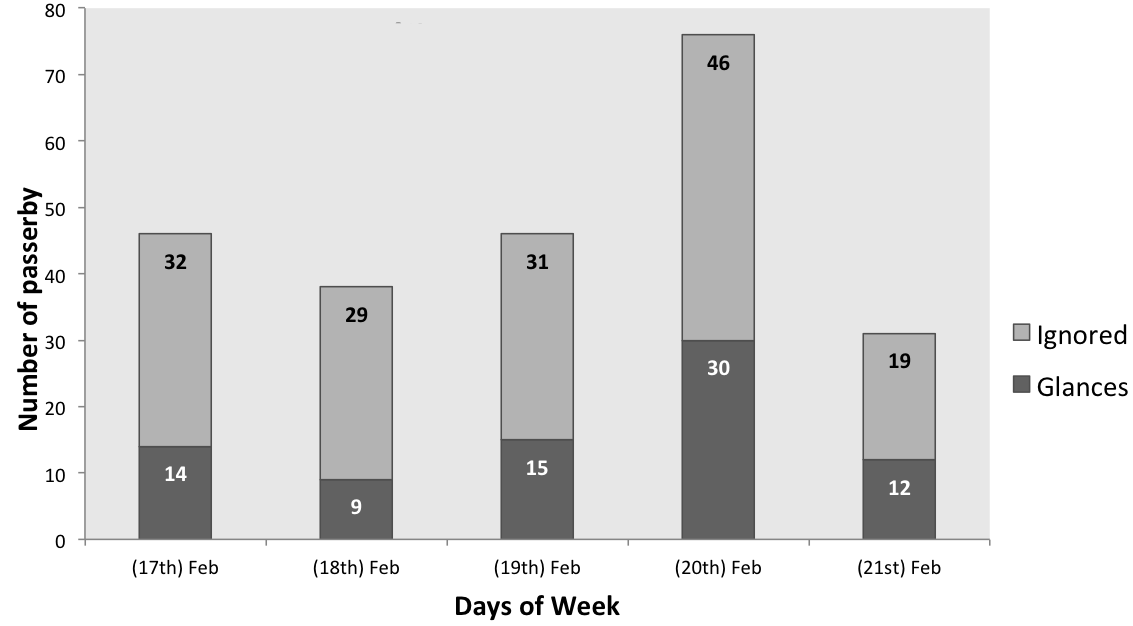
\includegraphics[width=110mm,height=60mm]{Figures/8/mobile_inter_findings/mobile_Inter_chart}%
    \caption{Mobile interactive attention level chart}%
    \label{fig:mobileattentionlevelchart}%
\end{figure}


\begin{figure}[H]
    \centering
    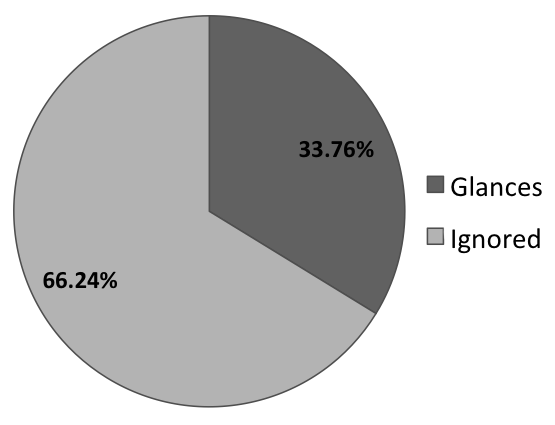
\includegraphics[width=110mm,height=60mm]{Figures/8/mobile_inter_findings/mobile_inter_percentage}
    \caption{Mobile interactive Attention level percentage}%
    \label{fig:bodyattentionlevelpercentage}%
\end{figure}


\item Engagement time

In average the engagement for the passerby took 21.70 seconds

\item Passerby and interactions


\begin{figure}[H]
    \centering
    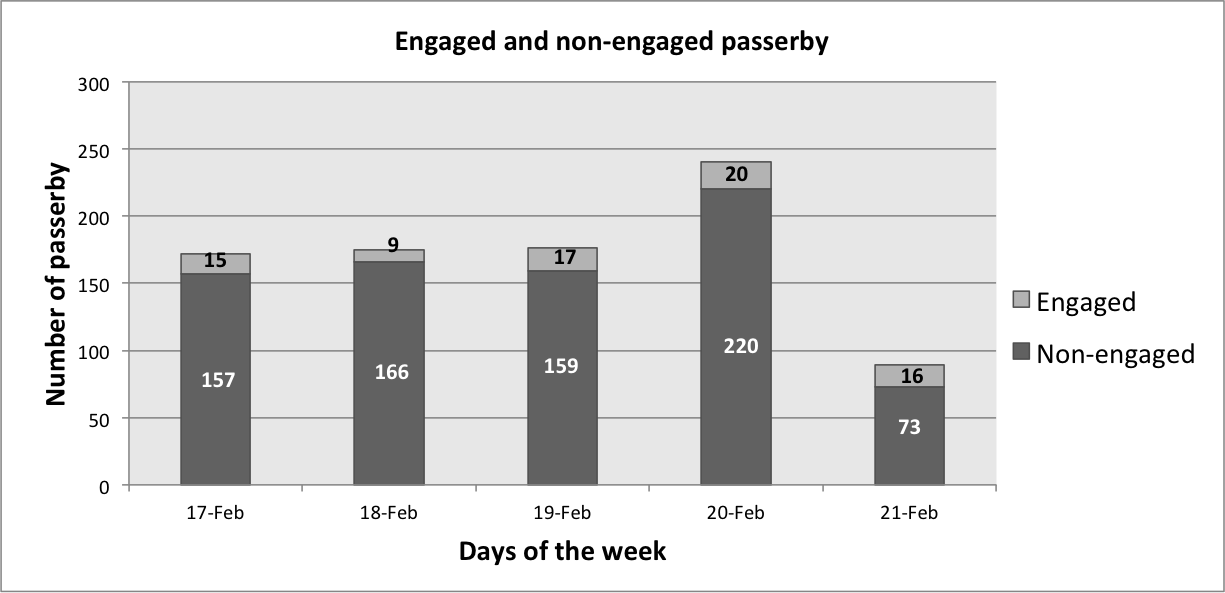
\includegraphics[width=110mm,height=60mm]{Figures/8/mobile_inter_findings/mobile_inter_engage_day}
    \caption{Mobile interactive Number of engaged passerby}%
    \label{fig:mobileengagedandengagedby}%
\end{figure}

\begin{figure}[H]
    \centering
    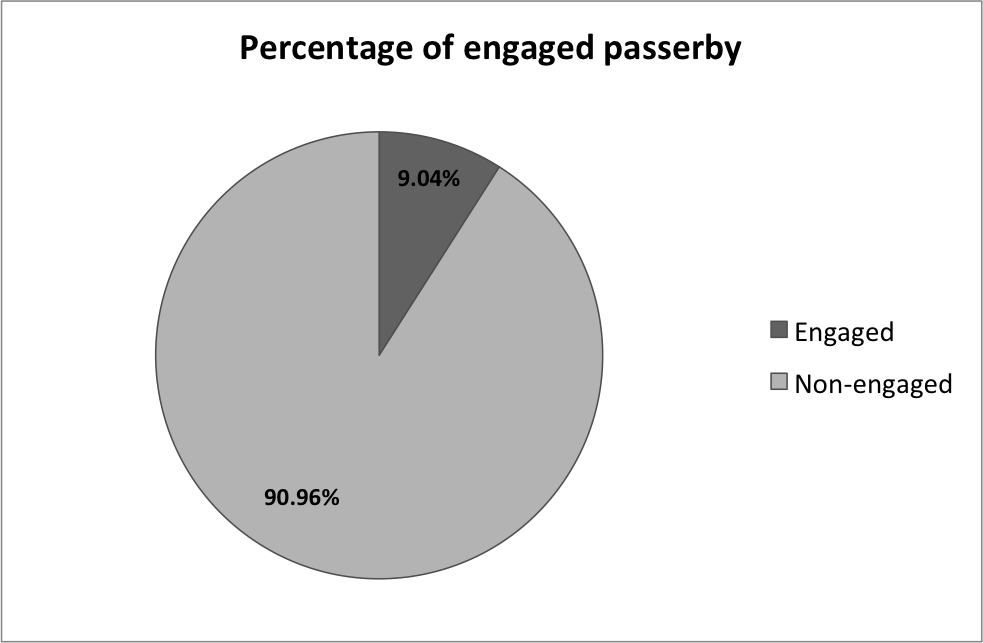
\includegraphics[width=110mm,height=60mm]{Figures/8/mobile_inter_findings/mobile_eng_percentage}
    \caption{Mobile interactive percentage of engaged passerby}%
    \label{fig:mobileengagedpasserbypercentage}%
\end{figure}

\item Landing and Honeypot effects

\begin{table}[H]
\caption{Mobile Interactive Landing and honeypot effect}
\label{tab:landingandhonypot_mobile}
\centering
\begin{tabular}{| l | c | c |}
\toprule
\tabhead{Days} & \tabhead{Landing effect} & \tabhead{Honeypot effect} \\
\midrule
\textbf{17 Feb}  & 0 &  1 \\
\textbf{18 Feb}  & 1 &  0 \\
\textbf{19 Feb}  & 2 &  0 \\
\textbf{20 Feb}  & 0 &  0 \\
\textbf{21 Feb}  & 1 &  1 \\
\bottomrule
\end{tabular}
\end{table}




\item Interview


\hilight{complete the interview report}



\item Note taking


see Appendix \ref{AppendixD}.11


\item Other observations

\end{enumerate}



\subsection{Comparison of advertisements}


\subsubsection{Hypothesis}


\begin{enumerate}
\item Attention Level measurements


\item Engagement time
\item Engagement phases
\item Passerby and interactions
\item Landing effect
\item Honeypot effect
\item Interview
\item Note taking
\item Other observations
\end{enumerate}
























































